The Application's workflow can be divided into three parts. The first part is quite simple, the user imports the video of his preference into the Application chooses the folder that he wants to save the results, and presses submit as it is shown in the figures above. 

\pagebreak

\begin{figure}[htp]
	\centering
	{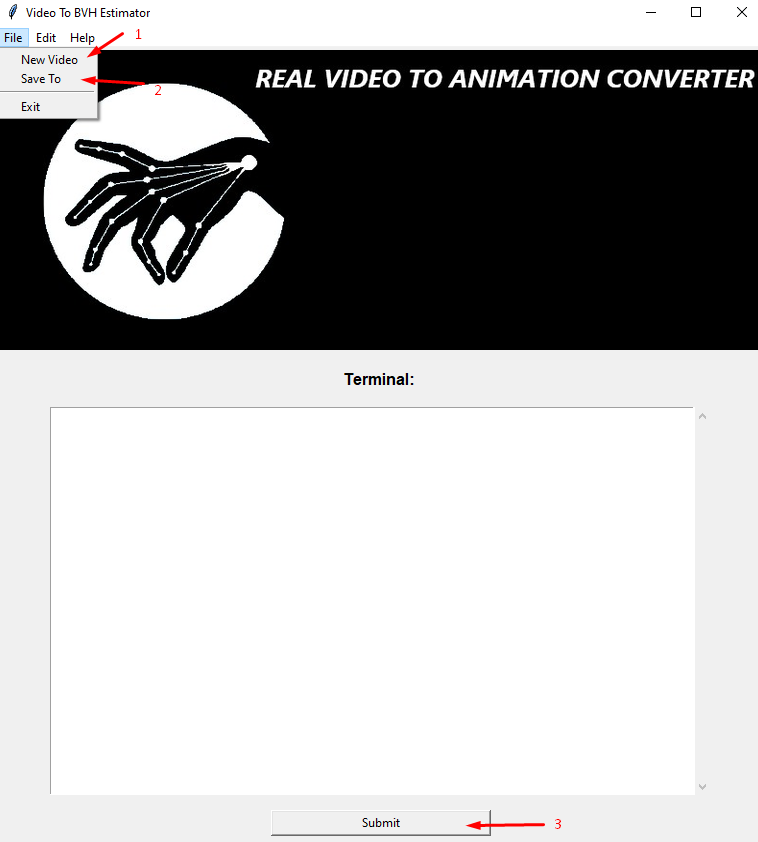
\includegraphics[height=9cm,width=0.48\linewidth]{figures/Requirements/Workflow1_1.png}}
	\hspace{1em}%
	{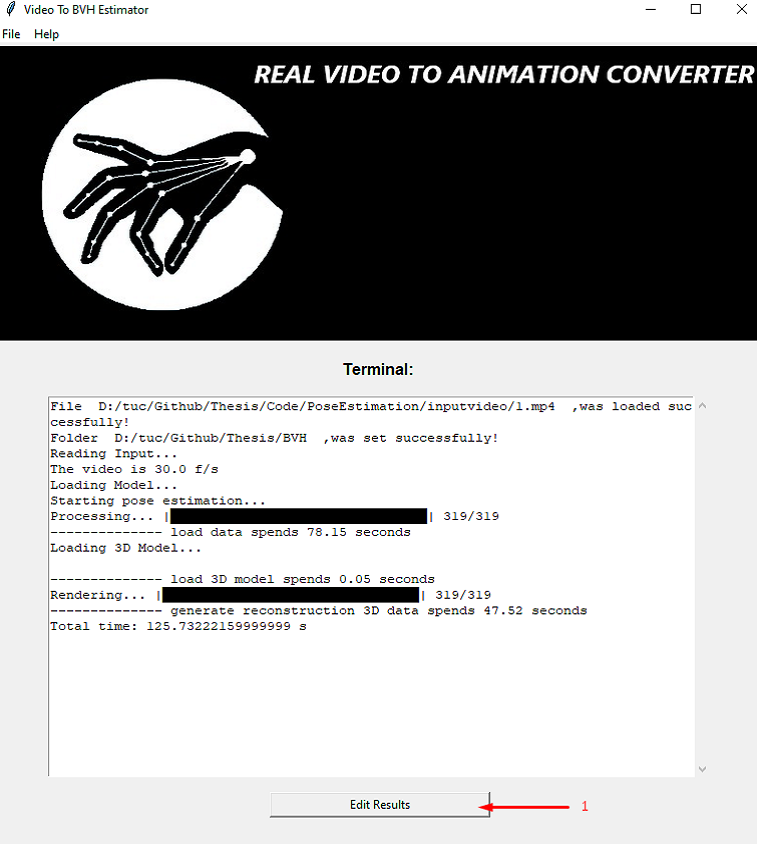
\includegraphics[height=9cm, width=0.48\linewidth]{figures/Requirements/Workflow1_2.png}}
	\captionsetup{labelformat=empty}
	\caption{Input Phase}
\end{figure}

In the above figure, in the left image, we show how to give new input to the Application. In the right image, we show the results that the user should see after a successful video to animation conversion as well as the way to go to the next panel.\\\\


 \begin{figure}[h]
	\centering
	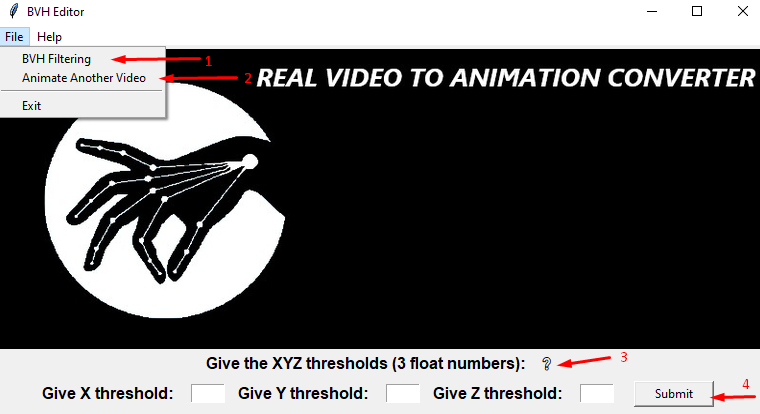
\includegraphics[width=0.55\textwidth]{figures/Requirements/Workflow2_1.png}
	\captionsetup{labelformat=empty}
	\caption{Editing Phase}
\end{figure}

\pagebreak

In the above figure, in the top image, the user can multiply with a number of his preference for each dimension in $R^3$. By doing so, he can increase or decrease the position speed. In the right image, the user can press the left button to filter the BVH motion data in order to reduce the noise, or can press the right button in order to return to the first panel and animate more videos. In addition, if the user does not understand something from the application, he can hover the mouse over the question marks to display some tips.\\\\


\begin{figure}[htp]
	\centering
	{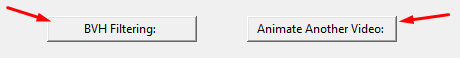
\includegraphics[height=10cm,width=0.48\linewidth]{figures/Requirements/Workflow2_2.png}}
	\hspace{1em}%
	{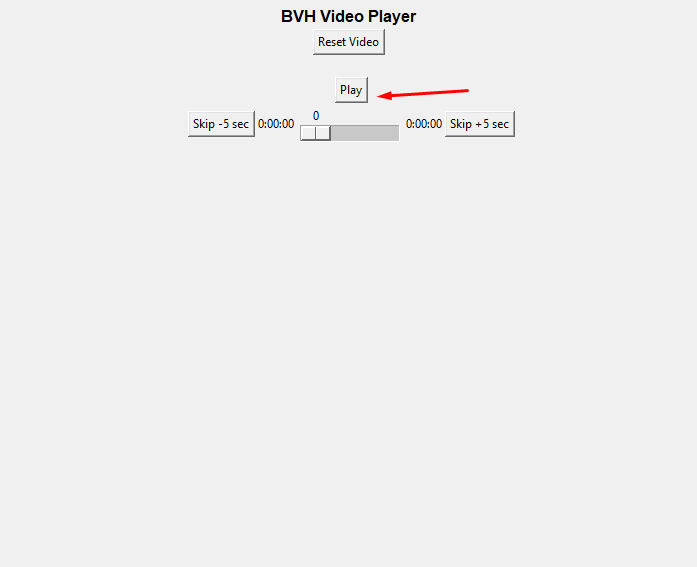
\includegraphics[height=10cm, width=0.48\linewidth]{figures/Requirements/Workflow2_3.png}}
	\captionsetup{labelformat=empty}
	\caption{BVH Video Player}
\end{figure}

The animators may change several things during this phase, so it would be very helpful if they could actually see the motion displayed in this panel. Therefore, if the pressed play, an mp4 of the motion starts playing. If the user changes something in the motion, either they filter the BVH or edit the position of the skeleton, in order to reload the mp4, they need to press reset the video. Unfortunately, this procedure is time-consuming, depending form the CPU the user has the speed of conversion from a BVH to an mp4, is about 10 frames per second.

\pagebreak

\begin{figure}[htp]
	\centering
	{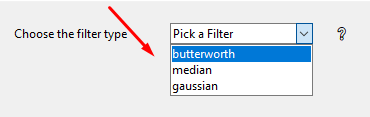
\includegraphics[height=3cm,width=0.48\linewidth]{figures/Requirements/Workflow3_1.png}}
	\hspace{1em}%
	{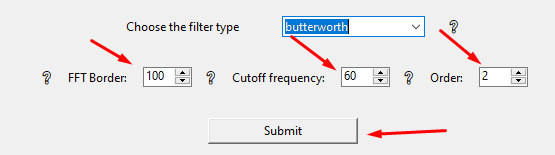
\includegraphics[height=3cm, width=0.48\linewidth]{figures/Requirements/Workflow3_2.png}}
	\captionsetup{labelformat=empty}
	\caption{Filtering Phase}
\end{figure}

In this phase the user can choose a filter of his preference, and insert the parameters that each filter need in order to work. The filter feature is added due to the fact that the estimation that the neural networks do, contain some noise, and these filters can significantly reduce it, or in some cases almost vanished it, which saves a lot of time from the animators.